\chapter{Демонстрация особенностей метода} 
\label{chapter4}

В данной главе экспериментальным способом на примере решения модельных задач показаны некоторые особенности разработанного метода. А именно, способность метода выбирать наиболее выгодные ФП на различных этапах оптимизации, тем самым повышая производительность ЭА, а также способность игнорировать такие ФП, применение которых приводит к ухудшению целевой ФП. Таким образом, выполняются требования, предъявляемые к методу в разд.~\ref{requirements}.

\section{Модельная задача min-max}
\label{model-problem}

	\subsection{Постановка задачи}
	Рассмотрим модельную задачу, на примере которой экспериментально проверена способность метода выбирать наиболее эффективные ФП на различных этапах оптимизации.
	Особь представлена битовой строкой длиной $n$, $x$ бит которой равны единице.
	Определим целевую ФП как
	\begin{equation}
	\label{eqn_target}
	g(x)=\left\lfloor \frac{x}{d} \right\rfloor.
	\end{equation}

	Вспомогательные функции имеют вид $h_1(x) = \min(x, p)$ и $h_2(x) = \max(x, p)$,
	где $p$ --- положительное целое число. Будем называть $p$ \emph{точкой переключения}.	
	Графики описанных функций представлены на рис.~\ref{pict:h1h2g}.

	Особенностью этой задачи является наличие точки переключения, позволяющее проверить способность метода динамически выбирать наиболее выгодную на данном этапе оптимизации функцию приспособленности. 
	Для особей,  число единиц в представлении которых меньше, чем точка переключения $p$, наиболее эффективно использовать вспомогательную функцию $h_1$ в качестве текущей. 
    Для остальных особей должна быть использована функция $h_2$. Ожидается, что в таком случае особи с более высокими значениями целевой функции $g$ будут выращены быстрее, 
    чем в случае использования самой целевой функции в качестве текущей. 
	
	\begin{figure}[h!]
		\center{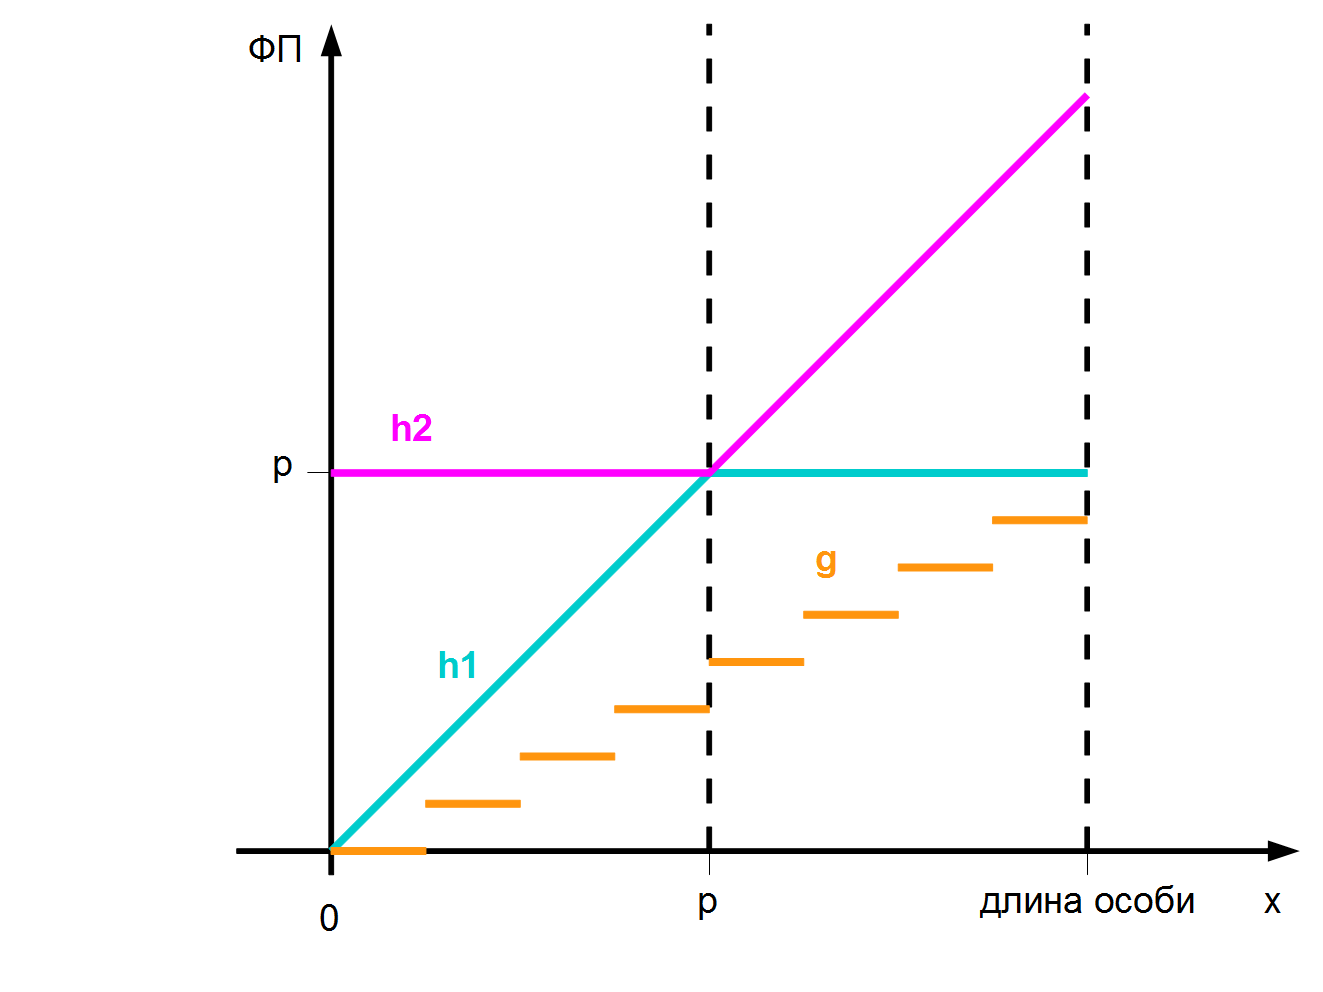
\includegraphics[width=0.6\textwidth]{h1h2g}}
		\caption{Функции приспособленности в модельной задаче}
		\label{pict:h1h2g}
	\end{figure}
		
	\subsection{Описание и результаты эксперимента}
	Был проведен ряд экспериментов, в ходе которых к решению модельной задачи применялись различные алгоритмы обучения с подкреплением, оптимизирующие генетический алгоритм (ГА). 
    Значения параметров ГА, использованные в экспериментах, представлены в табл.~\ref{experiment}. Было перебрано более тысячи различных комбинаций значений параметров обучения
    для каждого использованного алгоритма. Каждый алгоритм запускался 50 раз, и результаты, полученные с его помощью, усреднялись. Следует отметить, что наиболее выгодным значением дисконтного фактора (\ref{mark}) оказался ноль. Это указывает на то, что в данной задаче 
    информации о текущем состоянии среды достаточно для обучения и учет предыдущего опыта не требуется. 	
	
	\begin{table}[h!]
	\caption{Значения параметров, использованные в ходе эксперимента}
    \label{experiment}
	%\begin{center}
	\begin{tabular}{|l|l|} \hline
	Параметр & Значение \\ \hline
	Число запусков алгоритма & 50 \\ \hline
	Число особей в поколении & 100 \\ \hline
	Число поколений & 400 \\ \hline
	Коэффициент элитизма & 5 \\ \hline
	Вероятность кроссовера & 0.7 \\ \hline
	Вероятность мутации & 0.003 \\ \hline
	Длина особи & 400 \\ \hline
	Точка переключения & 266 \\ \hline
	Делитель $d$ & 10 \\ \hline
	\end{tabular}
	%\end{center}
	\end{table}
	
	Наилучшие результаты удалось получить, используя алгоритм обучения Q-learning c $\varepsilon$-жадной стратегией (\ref{strategy}). На рис.~\ref{pict:mm-dn-bounds} представлены графики зависимости 
    целевой ФП от номера поколения в случае использования метода, основанного на обучении, и обычного ГА. Можно видеть, что применение обучения позволяет гарантированно 
    вырастить идеальную особь менее, чем за 250 поколений. Использование обычного ГА, положенного в основу метода с обучением, не приводит к стабильному получению 
    идеальной особи в пределах использованного количества поколений, что проиллюстрировано на рис.~\ref{histogram}. Также на рис.~\ref{pict:mm-dn-bounds} находится диаграмма, отражающая число раз, когда была выбрана та или иная ФП. Отметим, что разработанный алгоритм успешно справился с выбором функций $h_1$ и $h_2$ на соответствующих этапах оптимизации.
	
	\begin{figure}[h!]
		\center{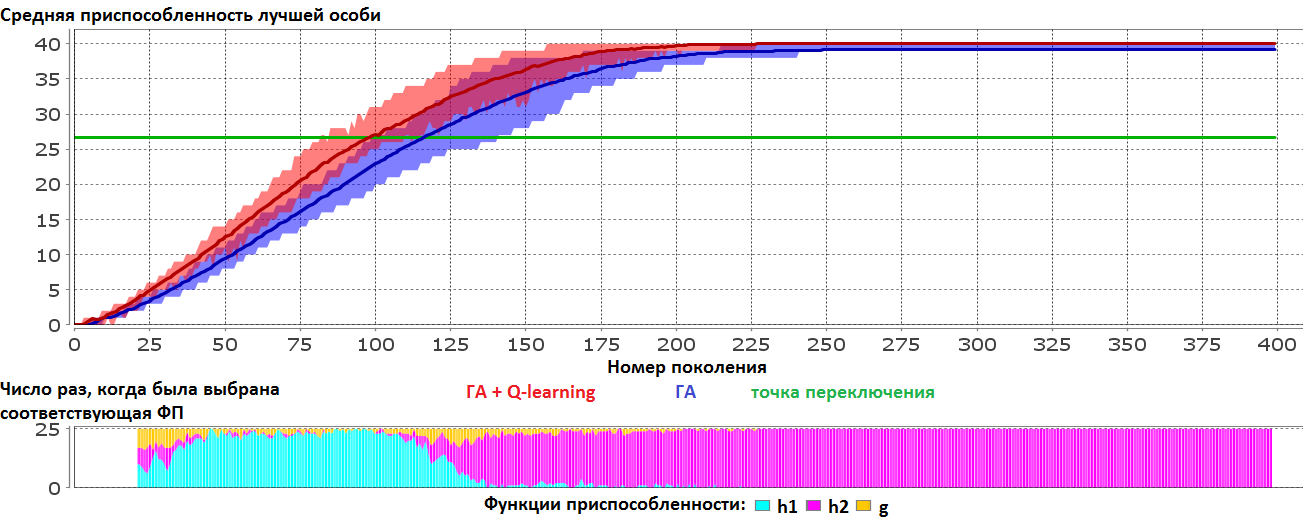
\includegraphics[width=\textwidth]{new-delayed}}
		\caption{Усредненные результаты решения модельной задачи min-max}
		\label{pict:mm-dn-bounds}
	\end{figure}
	
	\begin{figure}[h!]
		\center{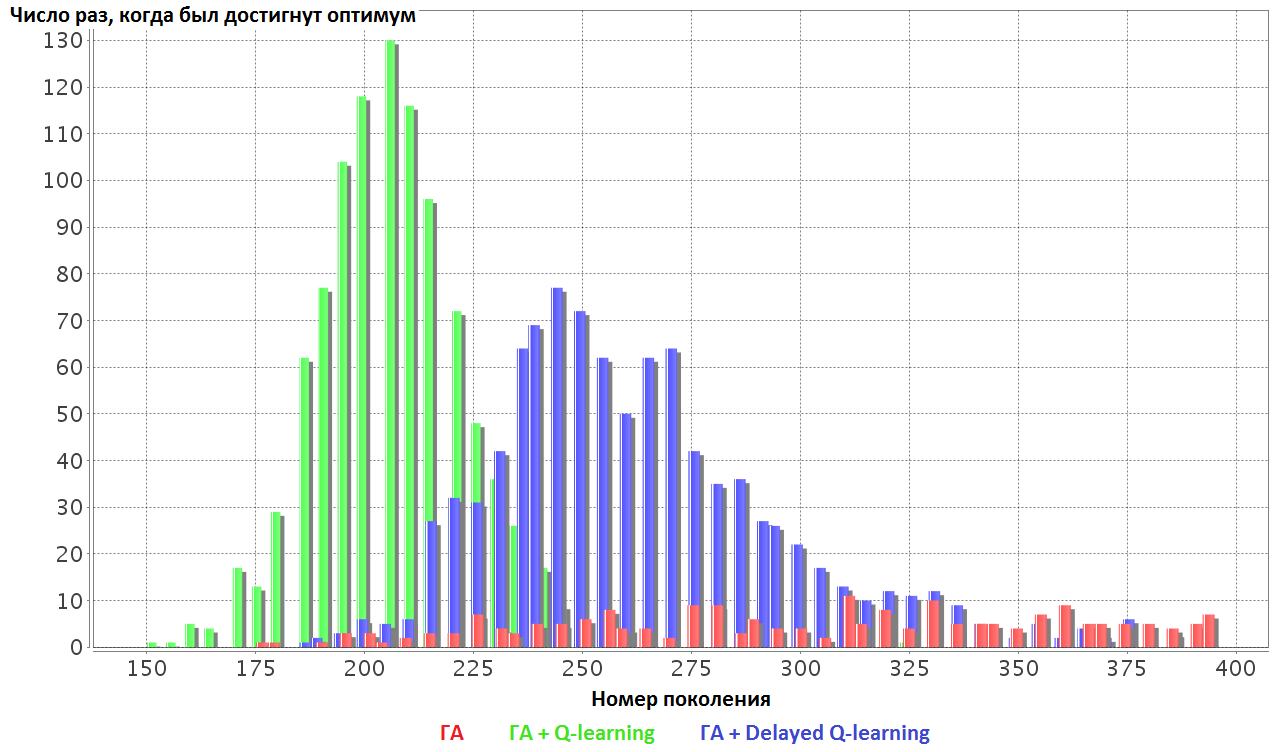
\includegraphics[width=\textwidth]{histogram1}}
		\caption{Распределение числа раз, когда было получено оптимальное решение задачи min-max, в зависимости от номера поколения}
		\label{histogram}
	\end{figure}
	
\section{Задача Royal Roads с мешающей ФП}

Рассмотрим модельную задачу, в которой оптимизация по единственной вспомогательной ФП приводит к быстрой убыли целевой. Экспериментально покажем, что определенные виды обучения способны справляться с решением такой задачи, выбирая целевую ФП. В качестве целевой ФП возьмем функцию Royal Roads \cite{mitchell-ga}. Пусть длина особи равна 64 битам. Выберем длину блока $b = 8$. Наличие очередного блока, заполненного $b$ единицами, увеличивает ФП на $b$. В качестве вспомогательной ФП будем использовать функцию, значение которой равно числу нулей, содержащихся в особи. 

В табл. \ref{royal} приведены результаты эксперимента по решению поставленной задачи. Усреднение производилось за 50 запусков каждого алгоритма. Выполнение алгоритма останавливалось при нахождении оптимума, либо при превышении максимального числа вычислений ФП, равного 500000. Число шагов в запусках, в которых не удалось получить оптимум, условно обозначено как бесконечность.

Можно видеть, что применение стратегии исследования среды по Больцману (\ref{strategy}) позволяет получить такую же производительность, что и без мешающей ФП. Использование алгоритма Delayed Q-learning, реализующего собственную стратегию исследования среды, также приводит к высоким результатам. Алгоритмы, использующие $\varepsilon$-жадную стратегию исследования среды значительно проигрывают упомянутым алгоритмам. Это можно объяснить тем, что для $\varepsilon$-жадной стратегии характерно существование постоянной вероятности $\varepsilon$, с которой выбирается случайное действие. Значит, в алгоритмах, использующих эту стратегию, всегда присутствует вероятность выбора мешающей ФП, равная $0,5\varepsilon$, что приводит к ухудшению целевой ФП. Заметим также, что установка нулевой вероятности выбора случайного действия в общем случае неэффективна (что подтверждается экспериментальными данными), так как подобный подход не позволяет агенту исследовать среду.

\begin{table}[ht]
\begin{center}
\caption{Результаты решения задачи Royal Roads} \label{royal}
\begin{tabular}{|p{4cm}|p{2cm}|p{2.5cm}|l|l|l|}
\hline
Алгоритм &\% успешных запусков & Шагов в успешных запусках (среднее) & Max шагов & Min шагов & $\sigma$\\
\hline
%\multicolumn{5}{|c|}{$(1+1)$ ЭС без мешающей ФП}\\ \hline
$(1+1)$ ЭС без мешающей ФП &100 & 6913,28 & 16033 & 2439 & 2925,07 \\ \hline
%\multicolumn{5}{|c|}{$(1+1)$ ЭС~+~Q-learning \cite{sutton} (больцмановская стратегия)}\\ \hline
ЭС~+~Q-learning \cite{sutton} (больцмановская стратегия) &100 & 6813,40 & 17252 & 2659 & 2999,60 \\ \hline
%\multicolumn{5}{|c|}{$(1+1)$ ЭС~+~Delayed \cite{delayed}}\\ \hline
$(1+1)$ ЭС~+~Delayed \cite{delayed} &88 & 8365,52 & $\infty$ & 3982 & 3216,13 \\ \hline
%\multicolumn{5}{|c|}{$(1+1)$ ЭС~+~R-learning \cite{r-learning} ($\varepsilon$-жадная стратегия)}\\ \hline
ЭС~+~R-learning \cite{r-learning} &100 & 69881,74 & 289936 & 5254 & 67990,07 \\ \hline
%\multicolumn{5}{|c|}{$(1+1)$ ЭС~+~Dyna \cite{sutton} ($\varepsilon$-жадная стратегия)}\\ \hline
ЭС~+~Dyna \cite{sutton} ($\varepsilon$-жадная стратегия) &26 & 5749,62 & $\infty$ & 2654 & 2056,78 \\ \hline
%\multicolumn{5}{|c|}{$(1+1)$ ЭС~+~Q-learning ($\varepsilon$-жадная стратегия)}\\ \hline
ЭС~+~Q-learning ($\varepsilon$-жадная стратегия) &24 & 6964,17 & $\infty$ & 3012 & 2256,70 \\ \hline
\end{tabular}
\end{center}
\end{table}

\section{Выводы по главе \protect\ref{chapter4}}
Описана модельная задача, позволяющая проверить работоспособность предлагаемого метода в случае, когда на различных этапах оптимизации выгодны различные вспомогательные ФП. 
Приведены результаты экспериментов, показывающие, что использование разработанного метода для решения описанной модельной задачи позволяет в 100\% запусков получать лучшую особь 
за конечное число поколений, в то время как с помощью ГА без обучения подобной производительности достичь не удается. В ходе эксперимента подтверждено, что разработанный метод 
динамически выбирает функцию приспособленности, наиболее выгодную на данном этапе.

Также описана задача, в которой оптимизация по вспомогательной ФП сильно ухудшает значение целевой ФП. Показано, что использование стратегии исследования среды по Больцману, а также алгоритма Delayed Q-learning, обладающего собственной стратегией исследования среды, позволяет получать такую же производительность, как в случае отсутствия мешающей ФП. Иначе говоря, обучение способно успешно игнорировать неэффективные вспомогательные ФП.
